Previous chapters described how to prepare Ubuntu, work with the Unity desktop and also learn to perform basic tasks. This chapter is all about personalising Ubuntu to your liking. In Ubuntu you can customize various aspects of your desktop like fonts, themes, wallpapers, Unity appearance etc. These are all illustrated in the sections below.

\section{Installing Lens \& Scopes} \index{Customisation!Additional Lenses and scopes}
In chapter \ref{chap:unity} the importance of the Unity dash was explained. The dash is the one stop place to quickly find your applications, file, folders, music and videos. However the search does not need to stop there. You can enhance the functionality of the dash by installing additional lenses and scopes. Additional lenses and scopes can be installed directly from the Ubuntu Software Center or by adding a Personal Package Archive (PPA) created by the community which includes many lenses. This sectional will illustrate both methods briefly. \\

\par \noindent Launch the Ubuntu Software Center as shown in chapter \ref{chap:software_management}. In the search you can search for additional lenses there and install them with just one click. However currently there are not many lenses which have been included in the Ubuntu Software Center. You can instead choose to install them the Scope Packagers PPA created by the community. This is illustrated in detail below. \\

\par \noindent The same instructions to add a PPA as explained in chapter \ref{chap:software_management} will be followed here. Let's start by first launching the Ubuntu Software Center. Then, open the Edit menu and click Software Sources. This is illustrated in figure \ref{fig:software-sources-menu}. In the software source dialog, choose other software and then click the add button. This is shown in figure \ref{fig:software-source-ppa}	and figure \ref{fig:software-source-ppa-add}. In the add dialog, enter the following \fbox{ppa:scopes-packagers/ppa}. You might have to restart your system for the software center to be refreshed and show the PPA. Once you have restarted the system, proceed to the Ubuntu Software Center. There as seen in figure \ref{fig:software-source-ppa-installapp}, you can install the additional lenses and scopes that you wish to install.

\section{3rd Party Applications} \label{sect:3rdpartyapps} 
Although the default Ubuntu install comes with an excellent selection of quality software out of the box, it is not possible to cater to the needs of all users, plus there are other limiting factors, such as the size of the distribution media (some software packages are very large), or licensing restrictions (some software requires that the user read and agree to the licence). \\

\par \noindent There are several methods available that may be used to install 3rd party applications. For example, suppose a user wishes to access a web site which requires Adobe Flash. A simple search in the Ubuntu Software Center will provide the desired result in this case. The Ubuntu Software Center has many of the most popular applications that typical users would seek. Click on the Install button, and Adobe Flash will be installed and configured. (Alternatively, some users may wish to perform installations using apt-get or aptitude via the Terminal.) On the other hand, users may wish to install software that is not provided in the standard Ubuntu software repositories (database), for various reasons. Sometimes, this may be due to the fact that the desired application is newer than the version provided in the Ubuntu Software Center. This is often handled by a Personal Package Archive, or PPA. One such example could be the latest version of Wine, which is a program that allows you to run Windows programs on other operating systems, including Ubuntu. Wine is available at http://www.winehq.org and clear, simple instructions for adding the Wine PPA (Stable or Development) to your Ubuntu Software Repositories are available at WineHQ. 

%\par \noindent Other times, there may not be a ready-made software package that is compatible with Ubuntu. Ubuntu uses the Debian package format (.deb), whereas other popular versions of Linux may use the Red Hat package format (.rpm). All is not lost, however - an application called alien sometimes allows the user to convert an .rpm package into a .deb package. Instructions for using alien on Ubuntu may be found at \href{https://help.ubuntu.com/community/RPM/AlienHowto}{here}. \\

%\par \noindent Note, however, that alien is not guaranteed to generate a working software package. Finally, a user may wish to run software for which there is no existing package at all - only the source code for the application. Although the steps required to build a package from source code are not difficult to follow, the task may be intimidating for some users. More details on building Ubuntu packages from source code may be found \href{http://developer.ubuntu.com/packaging/html/packaging-new-software.html}{here}. Again, there is no guarantee that the package will work as intended, but there is only one way to find out! So, as you can see, there are many ways to install 3rd party applications on Ubuntu - and if all else fails, remember to ask for help, as there is a good chance that someone has already done it before.

\section{Appearance} \index{Customisation!Appearance}
\subsection*{Wallpaper} \index{Customisation!Wallpaper}
The wallpaper can be easily changing by right-clicking anywhere on the desktop and pressing Change Desktop Background. On pressing the menu option, you are presented with Appearance dialog as seen in figure \ref{fig:appearance-look}. You can choose the wallpaper from the default collection of wallpapers as seen in the figure or you can choose your own wallpapers. You can also choose a wallpaper slide show represented by a clock (shown in figure \ref{fig:appearance-look} by a red box). This will then automatically change the wallpaper after a certain time interval.

\begin{figure}[h!]	
	\centering
	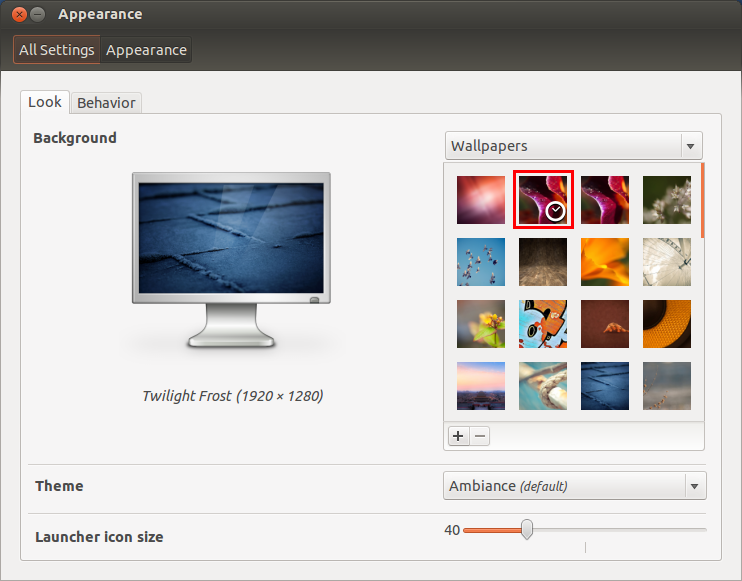
\includegraphics[width=300pt]{./images/customize-ubuntu/appearance-look.png}
	\caption{Appearance Dialog}	
	\label{fig:appearance-look}		
\end{figure}

\subsection*{Launcher} \index{Customisation!Launcher}
You also change the launcher appearance and behaviour in the appearance dialog. It can seen in figure \ref{fig:appearance-look}, the option to change the launcher icon size to your liking. You can also change the launcher behaviour by clicking on the behaviour tab in the appearance dialog. You are then presented with options as seen in figure \ref{fig:appearance-behavior}. You can choose to either have the launcher displayed always (default behaviour) or auto-hide it automatically. You can also adjust the reveal sensitivity which affects the pressure required to show the launcher. If the launcher appears too frequently by accident you can decrease the sensitivity and vice versa. 

\begin{figure}[h!]	
	\centering
	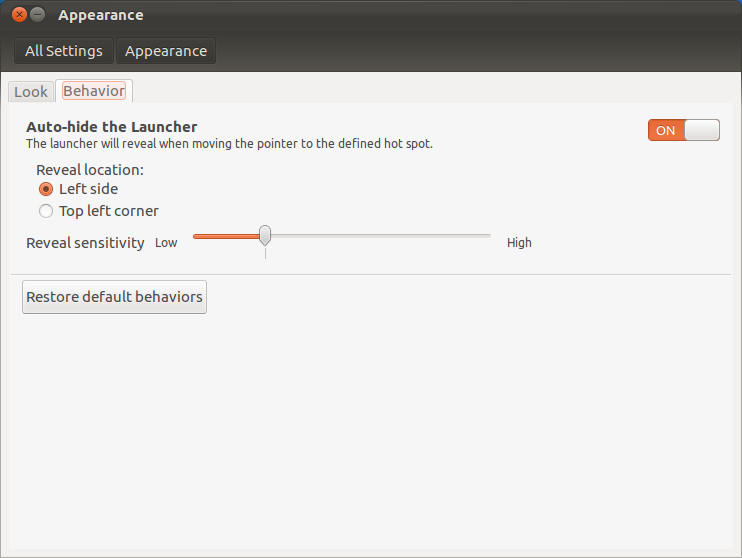
\includegraphics[width=250pt]{./images/customize-ubuntu/appearance-behavior.png}
	\caption{Appearance Dialog}	
	\label{fig:appearance-behavior}		
\end{figure}

%\subsection*{Fonts and Themes} \index{Customisation!Fonts and Themes}
 %This is explained in more detail in the previous section.
\newpage
\section{Privacy} \index{Privacy}
As you may have already noticed by now, the dash shows the recently used files, folders and applications. However, you can control what appears in the dash using the privacy settings in the system settings. Launch system settings using the dash or the launcher. The system settings is shown in figure \ref{fig:gcc}. The system settings is the central place to manage all the settings related to your system. \\

\begin{figure}[h!]	
	\centering
	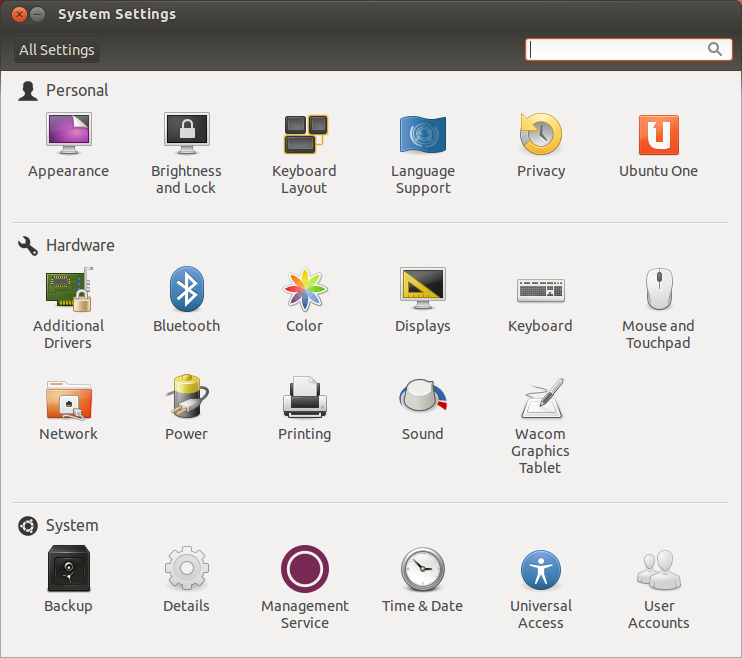
\includegraphics[width=300pt]{./images/customize-ubuntu/gcc.png}
	\caption{System Settings}	
	\label{fig:gcc}		
\end{figure}

\par \noindent In the system settings, click the privacy settings to launch the privacy settings manager as seen in figure \ref{fig:privacy}. Here you can choose to erase all the activity over a period of time. You can choose to delete all the history over the past hour, week or choose the time period yourself. \\

\begin{figure}[h!]	
	\centering
	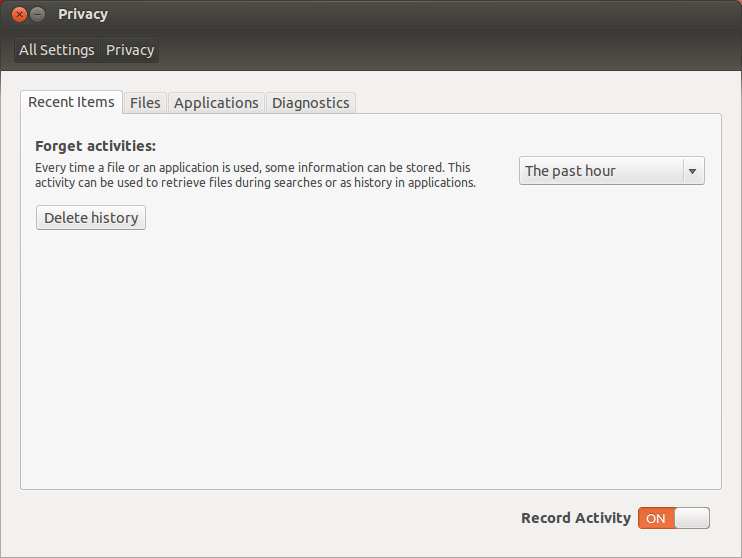
\includegraphics[width=300pt]{./images/customize-ubuntu/privacy.png}
	\caption{Privacy Manager}	
	\label{fig:privacy}		
\end{figure}

\par \noindent If you are interested to stop recording activity from certain types of files or specific folders, then click the files tab. This is shown in figure \ref{fig:privacy-files}. Here you can blacklist certain type of files such as video, email, text, image files etc. You can also blacklist a specific folder if required as well.\\

\begin{figure}[h!]	
	\centering
	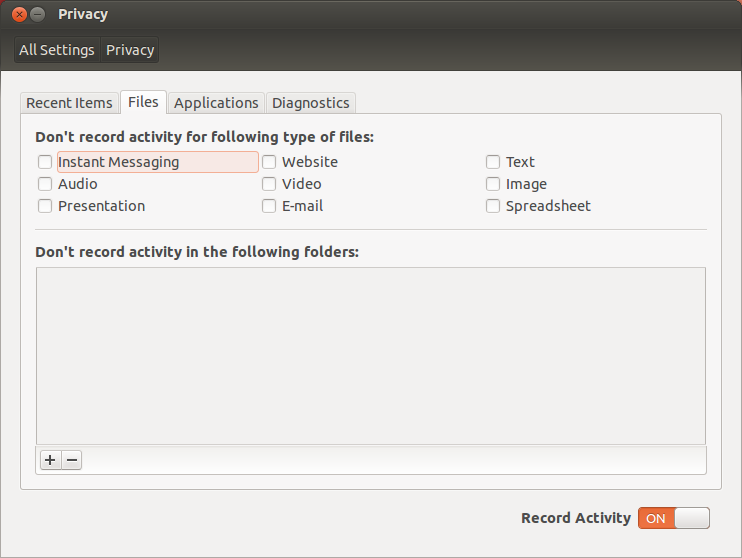
\includegraphics[width=300pt]{./images/customize-ubuntu/privacy-files.png}
	\caption{Privacy Manager}	
	\label{fig:privacy-files}		
\end{figure}

\par \noindent Finally, you can also manage privacy on an application basic by specifically blacklisting a certain application.  Note that blacklisting an application will not stop the recording of data performed by the application itself. For instance, if you blacklist Firefox, it will not show up in the recently used section in the dash but Firefox will still record your browsing history and other information. Click on the Applications tab as seen in figure \ref{fig:privacy-applications}. \\

\begin{figure}[h!]	
	\centering
	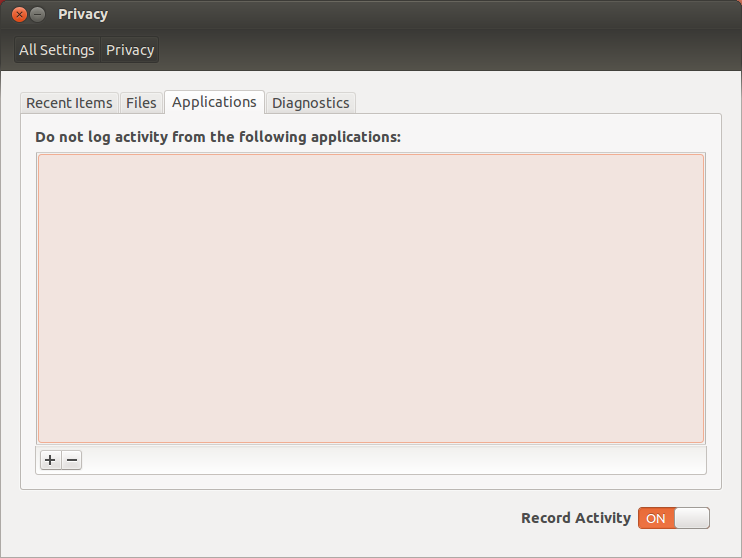
\includegraphics[width=300pt]{./images/customize-ubuntu/privacy-applications.png}
	\caption{Privacy Manager}	
	\label{fig:privacy-applications}		
\end{figure}
